\documentclass[aspectratio=1610,10pt]{beamer}

% Theme
% \usetheme{Madrid}
% \usecolortheme{default}

% Packages
\usepackage{amsmath, amssymb, amsfonts}
\usepackage{graphicx}
\usepackage{tikz}

% Title Info
\title{Heat Flow, Geometry, and Ricci Flow}
\author{
  Jack Bernstein-Sheehan and Hashem Damrah \\
  \small{Mentor: Arya Yae} \\
  \small{University of Oregon}
}
\date{\today}

\mode<presentation> { \setbeamercovered{transparent} }
\makeatletter
\def\beamerorig@set@color{%
  \pdfliteral{\current@color}%
  \aftergroup\reset@color
}
\def\beamerorig@reset@color{\pdfliteral{\current@color}}

\begin{document}
  \begin{frame}
    \titlepage
  \end{frame}

  %------------------------------------------------
  % Table of Contents
  %------------------------------------------------
  \begin{frame}{Overview of Presentation}
    \begin{itemize}
      \item Heat flow acts as a smoothing process.
      \item The behavior of heat depends on the underlying space.
      \item Geometry is encoded by a metric.
      \item Curvature measures how that geometry ``bends''.
      \item Ricci flow: evolve the metric the same way heat evolves temperature.
    \end{itemize}
  \end{frame}

  %------------------------------------------------
  % 1D Heat Flow & Concavity
  %------------------------------------------------
  \begin{frame}{1D Heat Flow and the Laplacian}
    Before looking at surfaces, consider the 1D heat equation:
    \[%
      \frac{\partial u}{\partial t} = u_{xx}
    .\]%
    \textbf{Why the second derivative?} It measures \emph{concavity}.
    \vspace{0.5cm}

    \begin{columns}
      \begin{column}{0.5\textwidth}
        \begin{itemize}
          \item If $u_{xx} < 0$ (concave down), temperature is a local maximum $\Rightarrow$ heat flows away ($u_t < 0$).
          \item If $u_{xx} > 0$ (concave up), temperature is a local minimum $\Rightarrow$ heat flows in ($u_t > 0$).
        \end{itemize}
      \end{column}
      \begin{column}{0.5\textwidth}
        \begin{center}
          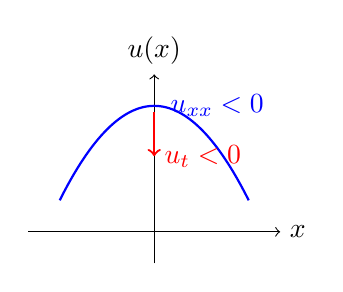
\begin{tikzpicture}[scale=0.8]
            \draw[->] (-2,0) -- (2,0) node[right] {$x$};
            \draw[->] (0,-0.5) -- (0,2.5) node[above] {$u(x)$};
            \draw[thick, blue] (-1.5,0.5) .. controls (-0.5,2.5) and (0.5,2.5) .. (1.5,0.5);
            \node[blue] at (1,2) {$u_{xx} < 0$};
            \draw[->, red, thick] (0,1.9) -- (0,1.2) node[right] {$u_t < 0$};
          \end{tikzpicture}
        \end{center}
      \end{column}
    \end{columns}
  \end{frame}

  %------------------------------------------------
  % Heat Equation (Cartesian)
  %------------------------------------------------
  \begin{frame}{Heat Equation in $\mathbb{R}^2$}
    We expand this to the classical heat equation in Cartesian coordinates:
    \[%
      \frac{\partial u}{\partial t} = u_{xx} + u_{yy} = \Delta u
    .\]%
    \begin{itemize}
      \item $u(x,y,t)$ = temperature.
      \item Heat flows from high to low.
      \item The Laplacian $\Delta u$ measures the ``average concavity'' in all directions.
    \end{itemize}
  \end{frame}

  %------------------------------------------------
  % Heat Equation (Polar)
  %------------------------------------------------
  \begin{frame}{Heat Equation in Polar Coordinates}
    In polar coordinates $(r,\theta)$, the Laplacian changes form. The heat equation becomes:
    \[
      \frac{\partial u}{\partial t} = \Delta_{\text{polar}} u = u_{rr} + \frac{1}{r}u_r + \frac{1}{r^2}u_{\theta\theta}
    \]
    \begin{itemize}
      \item Same physics, different coordinates.
      \item Extra terms come from geometry.
      \item Laplacian depends on how we measure space.
    \end{itemize}

    \begin{block}{Note}
      The Laplacian in Polar coordinates comes from the pushforward of the Cartesian Laplacian under the coordinate transformation. The extra terms arise because the basis vectors in polar coordinates are not constant and depend on position, leading to additional contributions when applying the chain rule.
    \end{block}
  \end{frame}

  %------------------------------------------------
  % Boundary Conditions
  %------------------------------------------------
  \begin{frame}{Boundary Conditions}
    To solve the heat equation on a bounded domain, we must specify what happens at the boundary $\partial M$.
    \vspace{0.5cm}

    \pause
    \begin{block}{Dirichlet Boundary Condition}
      Fixes the temperature at the boundary:
      \[%
        u(x,t) = C \quad \text{for}~x \in \partial M
      .\]%
      \emph{Physical meaning:} The boundary is held at a constant temperature (e.g., submerged in ice water).
    \end{block}

    \pause
    \begin{block}{Neumann Boundary Condition}
      Fixes the heat flux across the boundary:
      \[%
        \frac{\partial u}{\partial n}(x,t) = C \quad \text{for } x \in \partial M
      .\]%
      \emph{Physical meaning:} The boundary is perfectly insulated; no heat enters or escapes.
    \end{block}
  \end{frame}

  %------------------------------------------------
  % Metrics
  %------------------------------------------------
  \begin{frame}{What is a Metric?}
    \begin{itemize}
      \item A metric tells us how to measure \textbf{distance, angle, and area}.
      \item It encodes the geometry of the space.
    \end{itemize}

    \begin{block}{Examples}
      Flat (Cartesian):
      \[%
        ds^2 = dx^2 + dy^2
      .\]%
      Polar:
      \[%
        ds^2 = dr^2 + r^2 d\theta^2
      .\]%
    \end{block}
    \begin{itemize}
      \item Even flat space looks different under different coordinates.
      \item The metric determines how the second derivatives (and thus the Laplacian) are computed.
    \end{itemize}
  \end{frame}

  %------------------------------------------------
  % Laplacian and Metric
  %------------------------------------------------
  \begin{frame}{Laplacian Depends on Geometry}
    \begin{itemize}
      \item In general, we write the Laplacian as $\Delta_g$.
      \item The metric $g$ determines how we compute derivatives.
      \item Different metrics $\Rightarrow$ different Laplacians.
      \item Therefore: geometry directly affects heat flow.
    \end{itemize}

    \[%
      \text{metric} \rightarrow \text{Laplacian} \rightarrow \text{heat equation}
    .\]%
  \end{frame}

  %------------------------------------------------
  % Conformal Metrics & Weight Functions (Modified per Note 3)
  %------------------------------------------------
  \begin{frame}{Conformal Metrics and Weight Functions}
    \begin{block}{Definition}
      A metric $g$ is \emph{conformal} to the flat metric if there exists a strictly positive weight function $u(x,y)$ such that:
      \[%
        g = u(x,y)(dx^2 + dy^2)
      .\]%
    \end{block}

    \begin{itemize}
      \item In 1D, this looks like $g = u(x)dx^2$.
      \item The metric is obtained by scaling the flat metric.
      \item Angles are preserved, but lengths are rescaled by $\sqrt{u}$.
      \item Large $u$ stretches distances; small $u$ shrinks them.
      \item Geometry is encoded entirely in the weight function $u$.
    \end{itemize}
  \end{frame}

  %------------------------------------------------
  % Graph vs Surface
  %------------------------------------------------
  \begin{frame}{The Graph of $u$ vs. The Surface Itself}
    It is crucial to distinguish between the function $u(x,y)$ and the geometry it creates.

    \vspace{0.5cm}
    \textbf{The Graph of $u$:}
    \begin{itemize}
      \item The set of points $(x, y, u(x,y))$ in $\mathbb{R}^3$.
      \item The graph of $u$ can be used to produce an embedding of the 2d manifold in 2d.
    \end{itemize}

    \vspace{0.3cm}
    \textbf{The Surface defined by the metric $g = u(x,y)(dx^2 + dy^2)$:}
    \begin{itemize}
      \item You do not need a 3D ambient space to measure distances here.
      \item Walking on the $xy$-plane with a ``stretchy ruler'' defined by $u(x,y)$ is fundamentally different from walking on the 3D graph of $u$.
    \end{itemize}
  \end{frame}

  %------------------------------------------------
  % Fubini-Study
  %------------------------------------------------
  \begin{frame}{Fubini--Study Metric}
    A classic example of a conformal metric on the sphere $S^2 \cong \mathbb{C} \cup \{\infty\}$ is the Fubini-Study metric:
    \[%
      g_{FS} = \frac{4}{(1 + x^2 + y^2)^2} (dx^2 + dy^2)
    .\]%
    Here, our conformal weight function is:
    \[%
      u(x,y) = \frac{4}{(1 + x^2 + y^2)^2}
    .\]%
    This maps the flat plane to the standard round sphere via stereographic projection.
    \begin{figure}[H]
      \centering

      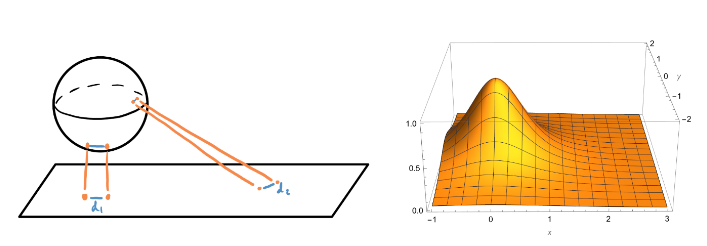
\includegraphics[width=0.8\textwidth]{./images/fubini-study-metric.png}

      \caption{Fubini-Study metric visualized as a surface in $\mathbb{R}^3$. The geometry of the surface encodes the curvature of the sphere.}
      \label{fig:}
    \end{figure}
  \end{frame}

  %------------------------------------------------
  % Curvature Formula & Calculation
  %------------------------------------------------
  \begin{frame}{Curvature of the Fubini-Study Metric}
    For a conformal metric $g = u(x,y)(dx^2 + dy^2)$, the Gaussian curvature $K$ is given by:
    \[%
      K = -\frac{1}{2u}\Delta (\log u)
    .\]%
    Let's calculate $K$ for Fubini-Study, where $u = 4(1+r^2)^{-2}$ and $r^2 = x^2+y^2$:
    \begin{align*}
      \log u &= \log 4 - 2\log(1+r^2) \\ \pause
      \Delta (\log u) &= \left(\frac{\partial^2}{\partial x^2} + \frac{\partial^2}{\partial y^2}\right) (\log 4 - 2\log(1+r^2)) \\ \pause
      \partial_x \log(1+r^2) &= \frac{2x}{1+r^2} \\ \pause
      \partial_{xx} \log(1+r^2) &= \partial{x} \left(\frac{2x}{1+r^2}\right) \\ \pause
                               &= \frac{2(1+r^2) - 4x^2}{(1+r^2)^2} = \frac{2-2x^2+2y^2}{(1+r^2)^2} \\ \pause
      \Delta \log(1+r^2) &= \frac{2-2x^2+2y^2 + 2-2y^2+2x^2}{(1+r^2)^2} = \frac{4}{(1+r^2)^2} \\ \pause
      \Delta (\log u) &= -2 \left( \frac{4}{(1+r^2)^2} \right) = -\frac{8}{(1+r^2)^2}
    .\end{align*}
  \end{frame}

  \begin{frame}{Curvature of the Fubini-Study Metric (Cont.)}
    Plugging the Laplacian back into our curvature formula:
    \begin{align*}
      K &= -\frac{1}{2u}\Delta (\log u) \\ \pause
        &= -\frac{1}{2 \left( \frac{4}{(1+r^2)^2} \right)} \left( -\frac{8}{(1+r^2)^2} \right) \\ \pause
        &= \frac{(1+r^2)^2}{8} \cdot \frac{8}{(1+r^2)^2} \\ \pause
        &= 1
    .\end{align*}
    The Fubini-Study metric describes a surface of \textbf{constant positive curvature} $K=1$, which perfectly matches our geometric intuition of a standard sphere.
  \end{frame}

  %------------------------------------------------
  % Connections and Geodesics
  %------------------------------------------------
  \begin{frame}{Connections and the Geodesic Equation}
    How do things move straight in a curved space? We need a \textbf{connection} ($\nabla$) to tell us how vectors change as we move.

    The metric determines the Levi-Civita connection, expressed via Christoffel symbols $\Gamma_{ij}^k$.

    \begin{block}{The Geodesic Equation}
      A path $\gamma(t)$ is a geodesic (a ``straight line'' in curved space) if its acceleration is zero with respect to the connection:
      \[%
        \nabla_{\dot{\gamma}} \dot{\gamma} = 0
      .\]%
      In local coordinates, this gives a system of 2nd-order ODEs:
      \[%
        \frac{d^2 \gamma^k}{dt^2} + \sum_{i,j} \Gamma_{ij}^k \frac{d\gamma^i}{dt} \frac{d\gamma^j}{dt} = 0
      .\]%
      Given a conformal metric, we can compute the geodesic equation as:
      \[%
        \nabla_{\dot{\gamma}} \dot{\gamma} = \ddot{\gamma} + \left(\partial_z \log(u^2)\right) \dot{\gamma}^2 = 0
      .\]%
    \end{block}
  \end{frame}

  %------------------------------------------------
  % Ricci Flow
  %------------------------------------------------
  \begin{frame}{The Ricci Flow Equation}
    Introduced by Richard Hamilton (1982), Ricci flow evolves the metric $g(t)$ to smooth out irregular curvature, governed by the Ricci curvature tensor $\text{Ric}$:
    \[%
      \frac{\partial}{\partial t} g_{ij} = -2\text{Ric}_{ij} + \rho g_{ij}
    .\]%
    For 2D surfaces, $\text{Ric}_{ij} = K g_{ij}$, where $K$ is the Gaussian curvature. The scalar $\rho$ dictates the type of flow:

    \begin{itemize}[<+->]
      \item \textbf{$\rho = 0$ (Unnormalized Ricci Flow):} The space shrinks or expands depending on the sign of curvature. Positive curvature shrinks to a point.
      \item \textbf{$\rho = \rho_t$ (Normalized Ricci Flow):} Here, $\rho_t$ is the time-dependent average curvature. This formulation preserves the total area of the surface as it evolves.
      \item \textbf{$\rho = \text{constant}$ (Yamabe Flow):} Evolving the metric by a constant scalar times the metric.
    \end{itemize}

    \begin{block}{Note}
      Flowing the weight function $u(x,y,t)$ smooths out bumps in the actual embedded manifold. This happens with bubbles in 3D space, as they round out as much as possible given whatever boundary constraints are imposed.
    \end{block}
  \end{frame}

  %------------------------------------------------
  % Ricci Flow (Surface Case)
  %------------------------------------------------
  \begin{frame}{Ricci Flow on Surfaces}
    For our 2D conformal metric $g = u(x,y,t)(dx^2 + dy^2)$, the unnormalized Ricci flow equation simplifies drastically.

    Since $\frac{\partial g}{\partial t} = -2Kg$, and $g = u(dx^2+dy^2)$, the weight function evolves according to:
    \[%
      \frac{\partial u}{\partial t} = -2Ku
    .\]%
    Substitute $K = -\frac{1}{2u}\Delta (\log u)$, we get:
    \[%
      \frac{\partial u}{\partial t} = -2 \left(-\frac{1}{2u}\Delta (\log u)\right) u = \Delta (\log u)
    ,\]%
    which is nice!
  \end{frame}
\end{document}
